\flushbottom


%%=============================================================================
%%=============================================================================
\chapter{Asymptotic Expansions}
\index{asymptotic expansions}


The more you sweat in practice, the less you bleed in battle.

\begin{flushright}
  -Navy Seal Saying
\end{flushright}

%%=============================================================================
\section{Asymptotic Relations}
\index{asymptotic relations}



\paragraph{The $\boldsymbol{\ll}$ and $\boldsymbol{\sim}$ symbols.}
First we will introduce two new symbols used in asymptotic relations.
\[ f(x) \ll g(x)\quad\mathrm{as}\ x \to x_0,\]
is read, ``$f(x)$ is much smaller than $g(x)$ as $x$ tends to $x_0$''.  
This means
\[\lim_{x \to x_0} \frac{f(x)}{g(x)} = 0.\]
The notation
\[ f(x) \sim g(x)\quad \mathrm{as}\ x \to x_0, \]
is read ``$f(x)$ is asymptotic to $g(x)$ as $x$ tends to $x_0$'';  which means
\[ \lim_{x \to x_0} \frac{f(x)}{g(x)} = 1.\]
A few simple examples are
\begin{itemize}
\item $-\e^x \gg x \quad \mathrm{as}\ x \to +\infty$
\item $\sin x \sim x \quad \mathrm{as}\ x \to 0$ 
\item $1/x \ll 1 \quad \mathrm{as}\ x \to +\infty$
\item $\e^{-1/x} \ll x^{-n} \quad \mathrm{as}\ x \to 0^+\ \mathrm{for all}\ n$
\end{itemize}


An equivalent definition of $f(x) \sim g(x)$ as $x \to x_0$ is
\[ f(x) - g(x) \ll g(x) \quad \mathrm{as}\ x \to x_0.\]
Note that it does not make sense to say that a function $f(x)$ 
is asymptotic to zero.  Using the above definition this would imply
\[ f(x) \ll 0 \quad \mathrm{as}\ x \to x_0.\]
If you encounter an expression like
$f(x) + g(x) \sim 0$, take this to mean $f(x) \sim - g(x)$.





\paragraph{The Big $\mathbf{\mathcal{O}}$ and Little $\mathbf{\mathsf{o}}$ 
  Notation.}
If $|f(x)| \leq m |g(x)|$ for some constant $m$ in some 
neighborhood of the point $x = x_0$, then we say that
\[ f(x) = \mathcal{O}(g(x)) \quad \mathrm{as}\ x \to x_0.\]
We read this as ``$f$ is big $\mathcal{O}$ of $g$ as $x$ goes to $x_0$''.
If $g(x)$ does not vanish, an equivalent definition is that
$f(x) / g(x)$ is bounded as $x \to x_0$.

If for any given positive $\delta$ there exists a neighborhood of $x=x_0$
in which $|f(x)| \leq \delta |g(x)|$ then 
\[ f(x) = \mathsf{o}(g(x)) \quad \mathrm{as}\ x \to x_0.\]
This is read, ``$f$ is little $o$ of $g$ as $x$ goes to $x_0$.''

For a few examples of the use of this notation,
\begin{itemize}
\item $ \e^{-x} = \mathsf{o}(x^{-n})$ as $x \to \infty$ for any $n$. 
\item $\sin x = \mathcal{O}(x)$ as $x \to 0$.
\item $\cos x - 1 = \mathsf{o}(1)$ as $x \to 0$.
\item $\log x = \mathsf{o}(x^\alpha)$ as $x \to +\infty$ 
  for any positive $\alpha$.
\end{itemize}



\paragraph{Operations on Asymptotic Relations.}
You can perform the ordinary arithmetic operations on asymptotic relations.
Addition, multiplication, and division are valid.

You can always integrate an asymptotic relation.  Integration is a smoothing
operation.  However, it is necessary to exercise some care.




\begin{Example}
  Consider 
  \[ f'(x) \sim \frac{1}{x^2} \quad \mathrm{as}\ x \to \infty.\]
  This does not imply that
  \[ f(x) \sim \frac{-1}{x} \quad \mathrm{as}\ x \to \infty.\]
  We have forgotten the constant of integration. Integrating the 
  asymptotic relation for $f'(x)$ yields
  \[ f(x) \sim \frac{-1}{x} + c \quad \mathrm{as}\ x \to \infty. \]
  If $c$ is nonzero then
  \[ f(x) \sim c \quad \mathrm{as}\ x \to \infty. \]
\end{Example}


It is not always valid to differentiate an asymptotic relation.  



\begin{Example}
  Consider $f(x) = \frac{1}{x} + \frac{1}{x^2} \sin(x^3)$.
  \[ f(x) \sim \frac{1}{x} \quad \mathrm{as}\ x \to \infty.\]
  Differentiating this relation yields
  \[f'(x) \sim -\frac{1}{x^2} \quad \mathrm{as}\ x \to \infty.\]
  However, this is not true since
  \begin{align*}
    f'(x)   &= -\frac{1}{x^2} - \frac{2}{x^3}\sin(x^3) + 2 \cos(x^3) \\
    &\not\sim -\frac{1}{x^2} \quad \mathrm{as}\ x \to \infty.
  \end{align*}
\end{Example}




\paragraph{The Controlling Factor.}
The controlling factor is the most rapidly varying factor in an asymptotic
relation.  Consider a function $f(x)$ that is asymptotic to $x^2 \e^x$
as $x$ goes to infinity.  The controlling factor is $\e^x$.  
For a few examples of this,
\begin{itemize}
\item $x \log x$ has the controlling factor $x$ as $x \to \infty$.
\item $x^{-2} \e^{1/x}$ has the controlling factor $\e^{1/x}$ as $x \to 0$.
\item $x^{-1} \sin x$ has the controlling factor $\sin x$ as $x \to \infty$.
\end{itemize}



\paragraph{The Leading Behavior.}
Consider a function that is asymptotic to a sum of terms.  
\[ f(x) \sim a_0(x) + a_1(x) + a_2(x) + \cdots, \quad \mathrm{as}\ x \to x_0.\]
where 
\[ a_0(x) \gg a_1(x) \gg a_2(x) \gg \cdots, \quad \mathrm{as}\ x \to x_0.\]
The first term in the sum is the leading order behavior.  For a few 
examples,
\begin{itemize}
\item For $\sin x \sim x - x^3/6 + x^5 / 120 - \cdots$ as $x \to 0$, the leading
  order behavior is $x$.
\item For $f(x) \sim \e^x(1 - 1/x + 1/x^2 - \cdots)$ as $x \to \infty$, the leading
  order behavior is $\e^x$.
\end{itemize}





%%============================================================================
\section{Leading Order Behavior of Differential Equations}
\index{leading order behavior!for differential equations}

It is often useful to know the leading order behavior of the solutions
to a differential equation.  If we are considering a regular point
or a regular singular point, the approach is straight forward.  We simply
use a Taylor expansion or the Frobenius method.  However, if we are
considering an irregular singular point, we will have to be a little
more creative.  Instead of an all encompassing theory like the
Frobenius method which always gives us the solution, 
we will use a heuristic approach that usually gives us the solution.







\begin{Example}
  Consider the Airy equation
  \[ y'' = x y. \]
  We
  \footnote{Using "We" may be a bit presumptuous on my part. Even if
    you don't particularly want to know how the solutions behave, I urge
    you to just play along.  This is an interesting section, I promise.}
  would like to know how the solutions of this equation behave as
  $x \to + \infty$.
  First we need to classify the point at infinity.  The change of variables
  \[ x = \frac{1}{t}, \quad y(x) = u(t), \quad \frac{\dd}{\dd x} = -t^2\frac{\dd}{\dd t},
  \quad \frac{\dd^2}{\dd x^2} = t^4 \frac{\dd^2}{\dd t^2} + 2t^3 \frac{\dd}{\dd t}\]
  yields
  \begin{gather*}
    t^4 u'' + 2 t^3 u' = \frac{1}{t} u \\
    u'' + \frac{2}{t} u' - \frac{1}{t^5} u = 0.
  \end{gather*}
  Since the equation for $u$ has an irregular singular point at zero, the equation for 
  $y$ has an irregular singular point at infinity.

  \paragraph{The Controlling Factor.}
  Since the solutions at irregular singular points often have exponential behavior, we
  make the substitution $y = \e^{s(x)}$ into the differential equation for $y$.
  \begin{gather*}
    \frac{\dd^2}{\dd x^2} \big[ \e^s \big] = x \e^s \\
    \big[s'' + (s')^2\big] \e^s = x \e^s \\
    s'' + (s')^2 = x
  \end{gather*}

  \paragraph{The Dominant Balance.}
  Now we have a differential equation for $s$ that appears harder to solve than our equation
  for $y$.  However, we did not introduce the substitution in order to obtain an equation 
  that we could solve exactly.  We are looking for an equation that we can solve
  approximately in the limit as $x \to \infty$.  If one of the terms in the equation for
  $s$ is much smaller that the other two as $x \to \infty$, then dropping that term and solving
  the simpler equation may give us an approximate solution.  If one of the terms in the 
  equation for $s$ is much smaller than the others then we say that the remaining
  terms form a \textbf{dominant balance} in the limit as $x \to \infty$.

  Assume that the $s''$ term is much smaller that the others, 
  $s'' \ll (s')^2, x$ as $x \to \infty$.  This gives us
  \begin{gather*}
    (s')^2 \sim x  \\
    s' \sim \pm \sqrt{x} \\
    s \sim \pm \frac{2}{3} x^{3/2} \quad \mathrm{as}\ x \to \infty.
  \end{gather*}
  Now let's check our assumption that the $s''$ term is small.  Assuming that we can 
  differentiate the asymptotic relation $s' \sim \pm \sqrt{x}$, we obtain 
  $s'' \sim \pm \frac{1}{2} x^{-1/2}$ as $x \to \infty$.
  \[ s'' \ll (s')^2, x \qquad \to \qquad x^{-1/2} \ll x \quad \mathrm{as}\ x \to \infty \]
  Thus we see that the behavior we found for $s$ is consistent with our assumption.
  The controlling factors for solutions to the Airy equation are $\exp(\pm \frac{2}{3}
  x^{3/2})$ as $x \to \infty$.

  \paragraph{The Leading Order Behavior of the Decaying Solution.}
  Let's find the leading order behavior as $x$ goes to infinity of the solution with the
  controlling factor $\exp(-\frac{2}{3} x^{3/2})$.  We substitute
  \[ s(x) = -\frac{2}{3} x^{3/2} + t(x), \qquad \mathrm{where}\ t(x) \ll x^{3/2}\ \mathrm{as}\ 
  x \to \infty \]
  into the differential equation for $s$.
  \begin{gather*}
    s'' + (s')^2 = x \\
    -\frac{1}{2} x^{-1/2} + t'' + (-x^{1/2} + t')^2 = x \\
    t'' + (t')^2 - 2 x^{1/2} t' - \frac{1}{2} x^{-1/2} = 0
  \end{gather*}
  Assume that we can differentiate $t \ll x^{3/2}$ to obtain
  \[ t' \ll x^{1/2}, \qquad t'' \ll x^{-1/2} \quad \mathrm{as}\ x \to \infty. \]
  Since $t'' \ll -\frac{1}{2} x^{-1/2}$ we drop the $t''$ term.  Also, 
  $t' \ll x^{1/2}$ implies that $(t')^2 \ll -2 x^{1/2} t'$, so we drop the
  $(t')^2$ term.  This gives us
  \begin{gather*}
    -2 x^{1/2} t' - \frac{1}{2} x^{-1/2} \sim 0 \\
    t' \sim -\frac{1}{4} x^{-1} \\
    t \sim -\frac{1}{4} \log x + c \\
    t \sim -\frac{1}{4} \log x \quad \mathrm{as}\ x \to \infty.
  \end{gather*}
  Checking our assumptions about $t$,
  \begin{alignat*}{3}
    t' &\ll x^{1/2} &\qquad &\to &\qquad x^{-1} &\ll x^{1/2} \\
    t'' &\ll x^{-1/2} &\qquad &\to &\qquad x^{-2} &\ll x^{-1/2}
  \end{alignat*}
  we see that the behavior of $t$ is consistent with our assumptions.

  So far we have
  \[ y(x) \sim \exp \left( -\frac{2}{3} x^{3/2} - \frac{1}{4} \log x + u(x) 
  \right) \quad \mathrm{as}\ x \to \infty, \]
  where $u(x) \ll \log x$ as $x \to \infty$.
  To continue, we substitute $t(x) = -\frac{1}{4} \log x + u(x)$ into the 
  differential equation for $t(x)$.
  \begin{gather*}
    t'' + (t')^2 - 2 x^{1/2} t' - \frac{1}{2} x^{-1/2} = 0 \\
    \frac{1}{4} x^{-2} + u'' + \left(-\frac{1}{4} x^{-1} + u' \right)^2
    - 2 x^{1/2} \left( -\frac{1}{4} x^{-1} + u' \right) 
    -\frac{1}{2} x^{-1/2} = 0 \\
    u'' + (u')^2 + \left( -\frac{1}{2} x^{-1} - 2 x^{1/2} \right) u' 
    + \frac{5}{16} x^{-2} = 0
  \end{gather*}
  Assume that we can differentiate the asymptotic relation for $u$ to obtain
  \[ u' \ll x^{-1}, \qquad u'' \ll x^{-2} \quad \mathrm{as}\ x \to \infty. \]
  We know that $-\frac{1}{2} x^{-1} u' \ll -2 x^{1/2} u'$.  Using
  our assumptions,
  \begin{alignat*}{3}
    u'' &\ll x^{-2} &\qquad &\to &\qquad u'' &\ll \frac{5}{16} x^{-2} \\
    u' &\ll x^{-1} &\qquad &\to &\qquad (u')^2 &\ll \frac{5}{16} x^{-2}.
  \end{alignat*}
  Thus we obtain
  \begin{gather*}
    -2 x^{1/2} u' + \frac{5}{16} x^{-2} \sim 0 \\
    u' \sim \frac{5}{32} x^{-5/2} \\
    u \sim -\frac{5}{48} x^{-3/2} + c \\
    u \sim c \quad \mathrm{as}\ x \to \infty.
  \end{gather*}
  Since $u = c + \mathsf{o}(1)$, $\e^u = \e^c + \mathsf{o}(1)$.  
  The behavior of $y$ is
  \[ y \sim x^{-1/4} \exp\left(-\frac{2}{3} x^{3/2} \right)(\e^c + \mathsf{o}(1))
  \quad \mathrm{as}\ x \to \infty. \]
  Thus the full leading order behavior of the decaying solution is
  \[ \boxed{ y \sim (\mathrm{const})x^{-1/4} \exp\left(-\frac{2}{3} x^{3/2} \right)
    \quad \mathrm{as}\ x \to \infty.} \]
  You can show that the leading behavior of the exponentially growing solution
  is

  \[ y \sim (\mathrm{const})x^{-1/4} \exp\left(\frac{2}{3} x^{3/2} \right)
  \quad \mathrm{as}\ x \to \infty. \]
\end{Example}












\begin{Example}\textbf{The Modified Bessel Equation.}
  Consider the modified Bessel equation
  \[ x^2 y'' + x y' - (x^2 + \nu^2) y = 0.\]
  We would like to know how the solutions of this equation behave as
  $x \to + \infty$.
  First we need to classify the point at infinity.  The change of variables
  $x = \frac{1}{t}$, $y(x) = u(t)$ yields
  \begin{gather*}
    \frac{1}{t^2}(t^4 u'' + 2t^3 u') + \frac{1}{t}(-t^2 u')
    - \left(\frac{1}{t^2} + \nu^2\right)u = 0 \\
    u'' + \frac{1}{t} u' - \left(\frac{1}{t^4} + \frac{\nu^2}{t^2}\right)u = 0
  \end{gather*}
  Since $u(t)$ has an irregular singular point at $t=0$, $y(x)$ has an
  irregular singular point at infinity.

  \paragraph{The Controlling Factor.}
  Since the solutions at irregular singular points often have 
  exponential behavior, we make
  the substitution $y = \e^{s(x)}$ into the differential equation for $y$.
  \begin{gather*}
    x^2(s'' + (s')^2) \e^s + x s' \e^s - (x^2 + \nu^2) \e^s = 0 \\
    s'' + (s')^2  + \frac{1}{x} s'  - (1 + \frac{\nu^2}{x^2}) = 0
  \end{gather*}
  We make the assumption that $s'' \ll (s')^2$ as $x \to \infty$ and we
  know that $\nu^2/x^2 \ll 1$ as $x \to \infty$.  Thus we drop these
  two terms from the equation to obtain an approximate equation for $s$.
  \[ (s')^2 + \frac{1}{x} s' - 1 \sim 0 \] 
  This is a quadratic equation for $s'$, so we can solve it exactly.  However,
  let us try to simplify the equation even further.  Assume that as $x$
  goes to infinity one of the three terms is much smaller that the other 
  two.  If this is the case, there will be a balance between the two
  dominant terms and we can neglect the third.
  Let's check the three possibilities.
  \begin{enumerate}
  \item 
    \[ 1\ \mathrm{is small.} \qquad \to \qquad
    (s')^2 + \frac{1}{x}s' \sim 0 \qquad \to \qquad 
    s' \sim - \frac{1}{x}, 0 \]  
    $1 \not\ll \frac{1}{x^2}, 0$ as $x \to \infty$ 
    so this balance is inconsistent.
  \item
    \[ \frac{1}{x} s'\ \mathrm{is small.} \qquad \to \qquad
    (s')^2 - 1 \sim 0 \qquad \to \qquad s' \sim \pm 1 \]
    This balance is consistent as $\frac{1}{x} \ll 1$ as $x \to \infty$.
  \item
    \[ (s')^2\ \mathrm{is small.} \qquad \to \qquad
    \frac{1}{x} s' - 1 \sim 0 \qquad \to \qquad s' \sim x \]
    This balance is not consistent as $x^2 \not\ll 1$ as $x \to \infty$.
  \end{enumerate}

  The only dominant balance that makes sense leads to $s' \sim \pm 1$ as
  $x \to \infty$.  Integrating this relationship,
  \begin{align*}
    s &\sim \pm x + c \\
    &\sim \pm x \quad \mathrm{as}\ x \to \infty.
  \end{align*}
  Now let's see if our assumption that we made to get the simplified equation
  for $s$ is valid.  Assuming that we can differentiate $s' \sim \pm 1$,
  $s'' \ll (s')^2$ becomes
  \begin{align*}
    \frac{\dd}{\dd x} \big[\pm 1 + \mathsf{o}(1)\big] &\ll \big[\pm 1 
    + \mathsf{o}(1)\big]^2 \\
    0 + \mathsf{o}(1/x) &\ll 1
  \end{align*}
  Thus we see that the behavior we obtained for $s$ is consistent with 
  our initial assumption.

  We have found two controlling factors, $\e^x$ and $\e^{-x}$.  This is a good
  sign as we know that there must be two linearly independent solutions
  to the equation.




  \paragraph{Leading Order Behavior.}
  Now let's find the full leading behavior of the solution with the
  controlling factor $\e^{-x}$.  In order to find a better
  approximation for $s$, we substitute $s(x) = -x + t(x)$,
  where $t(x) \ll x$ as $x \to \infty$, into the differential
  equation for $s$. 
  \begin{gather*}
    s'' + (s')^2 + \frac{1}{x} s' - \left(1 + \frac{\nu^2}{x^2}\right) = 0 \\
    t'' + (-1 + t')^2 + \frac{1}{x}(-1 + t') - \left(1 + \frac{\nu^2}{x^2}\right) 
    = 0 \\
    t'' + (t')^2 + \left(\frac{1}{x} - 2\right)t'
    - \left(\frac{1}{x} + \frac{\nu^2}{x^2}\right) = 0 
  \end{gather*}

  We know that $\frac{1}{x} \ll 2$ and $\frac{\nu^2}{x^2} \ll \frac{1}{x}$
  as $x \to \infty$.  Dropping these terms from the equation yields
  \[ t'' + (t')^2 - 2t' - \frac{1}{x} \sim 0.\]
  Assuming that we can differentiate the asymptotic relation for $t$, we obtain
  $t' \ll 1$ and $t'' \ll \frac{1}{x}$ as $x \to \infty$.  We
  can drop $t''$. Since $t'$ vanishes as $x$ goes to infinity, $(t')^2 \ll t'$.
  Thus we are left with 
  \[ - 2t' - \frac{1}{x} \sim 0, \quad \mathrm{as}\ x \to \infty.\]
  Integrating this relationship,
  \begin{align*}
    t &\sim -\frac{1}{2} \log x + c \\
    &\sim -\frac{1}{2} \log x \quad \mathrm{as}\ x \to \infty.
  \end{align*}
  Checking our assumptions about the behavior of $t$,
  \begin{alignat*}{2}
    t' &\ll 1 \qquad &\to \qquad -\frac{1}{2x} &\ll 1 \\
    t'' &\ll \frac{1}{x} \qquad &\to \qquad \frac{1}{2x^2} &\ll \frac{1}{x}
  \end{alignat*}
  we see that the solution is consistent with our assumptions.

  The leading order behavior to the solution with controlling factor $\e^{-x}$ is
  \[ y(x) \sim \exp\left(-x - \frac{1}{2} \log x + u(x) \right)
  = x^{-1/2} \e^{-x + u(x)} \quad \mathrm{as}\ x \to \infty,\]
  where $u(x) \ll \log x$.
  We substitute $t = -\frac{1}{2} \log x + u(x)$ into the differential equation
  for $t$ in order to find the asymptotic behavior of $u$.
  \begin{gather*}
    t'' + (t')^2 + \left(\frac{1}{x} - 2\right) t' 
    - \left(\frac{1}{x} + \frac{\nu^2}{x^2}\right) = 0\\
    \frac{1}{2x^2} + u'' + \left(-\frac{1}{2x} + u'\right)^2 
    + \left(\frac{1}{x} - 2\right)
    \left(-\frac{1}{2x} + u'\right) 
    - \left(\frac{1}{x} + \frac{\nu^2}{x^2}\right) = 0 \\
    u'' + (u')^2 - 2u' + \frac{1}{4x^2} - \frac{\nu^2}{x^2} = 0
  \end{gather*}
  Assuming that we can differentiate the asymptotic relation for $u$,
  $u' \ll \frac{1}{x}$ and $u'' \ll \frac{1}{x^2}$ as $x \to \infty$.
  Thus we see that we can neglect the $u''$ and $(u')^2$ terms.
  \[ -2 u' + \left(\frac{1}{4} - \nu^2\right)\frac{1}{x^2} \sim 0 \]
  \begin{align*}
    u' &\sim \frac{1}{2} \left(\frac{1}{4} - \nu^2\right) \frac{1}{x^2} \\
    u &\sim \frac{1}{2} \left(\nu^2 -  \frac{1}{4} \right) \frac{1}{x} + c \\
    u &\sim c \quad \mathrm{as}\ x \to \infty
  \end{align*}
  Since $u = c + \mathsf{o}(1)$, we can expand $\e^u$ as $\e^c + \mathsf{o}(1)$.  
  Thus we can write the leading order behavior as
  \[ y \sim x^{-1/2} \e^{-x} (\e^c + \mathsf{o}(1)).\]
  Thus the full leading order behavior is
  \[ \boxed{y \sim (\mathrm{const})x^{-1/2} \e^{-x} \quad \mathrm{as}\ x \to \infty.}\]
  You can verify that the solution with the controlling factor $\e^x$ has
  the leading order behavior
  \[ y \sim (\mathrm{const}) x^{-1/2} \e^x \quad \mathrm{as}\ x \to \infty. \]

  Two linearly independent solutions to the modified Bessel equation are the 
  modified Bessel functions, $I_\nu(x)$ and $K_\nu(x)$.  These functions
  have the asymptotic behavior
  \[ I_\nu(x) \sim \frac{1}{\sqrt{2\pi x}} \e^x, 
  \qquad K_\nu(x) \sim \frac{\sqrt{\pi}}{\sqrt{2x}}
  \e^{-x}\quad \mathrm{as}\ x \to \infty. \]
  In Figure~\ref{besselk0} $K_0(x)$ is plotted in a solid line and 
  $\frac{\sqrt{\pi}}{\sqrt{2x}} \e^{-x}$ is plotted in a dashed line.  We see
  that the leading order behavior of the solution as $x$ goes to infinity
  gives a good approximation to the behavior even for fairly small values
  of $x$.

  \begin{figure}[h!]
    \begin{center}
      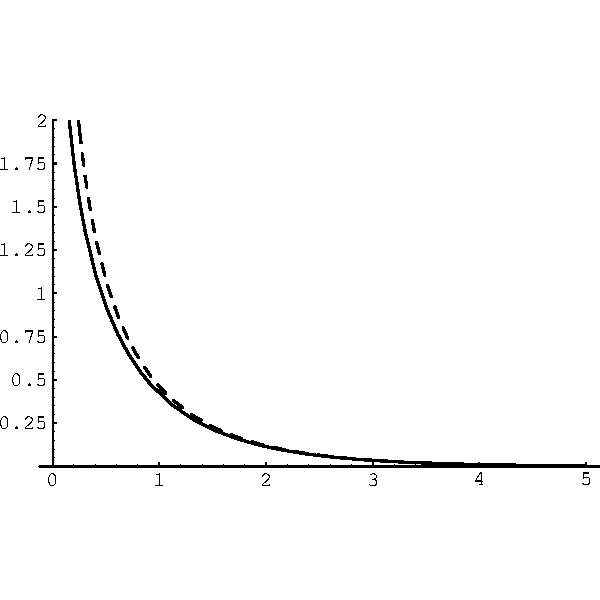
\includegraphics[width=0.6\textwidth]{ode/asymptotic/besselk0}
    \end{center}
    \caption{Plot of the modified Bessel function and its leading order 
      behavior.}
    \label{besselk0}
  \end{figure}

\end{Example}





















%%=============================================================================
\section{Integration by Parts}
\index{asymptotic expansions!integration by parts}

\begin{Example}
  \label{error_function}
  The complementary error function
  \[ \erfc(x) = \frac{2}{\sqrt{\pi}} \int_x^\infty \e^{-t^2}\,dt\]
  is used in statistics for its relation to the normal probability distribution.
  We would like to find an approximation to $\erfc(x)$ for large $x$.
  Using integration by parts,
  \begin{align*}
    \erfc(x)
    &= \frac{2}{\sqrt{\pi}}\int_x^\infty \left(\frac{-1}{2t}\right)
    \left(-2 t \e^{-t^2}\right)\,dt \\
    &= \frac{2}{\sqrt{\pi}}\left[\frac{-1}{2t}\e^{-t^2}\right]_x^\infty - 
    \frac{2}{\sqrt{\pi}}\int_x^\infty
    \frac{1}{2}t^{-2} \e^{-t^2}\,dt \\
    &= \frac{1}{\sqrt{\pi}}x^{-1} \e^{-x^2} - 
    \frac{1}{\sqrt{\pi}}\int_x^\infty t^{-2} \e^{-t^2}\,dt. 
  \end{align*}
  We examine the residual integral in this expression.
  \begin{align*}
    \frac{1}{\sqrt{\pi}} \int_x^\infty t^{-2} \e^{-t^2}\,dt
    &\leq \frac{-1}{2\sqrt{\pi}} x^{-3} \int_x^\infty -2t \e^{-t^2}\,dt \\
    &= \frac{1}{2\sqrt{\pi}} x^{-3} \e^{-x^2}.
  \end{align*}
  Thus we see that
  \[\frac{1}{\sqrt{\pi}}x^{-1} \e^{-x^2} \gg 
  \frac{1}{\sqrt{\pi}}\int_x^\infty t^{-2} \e^{-t^2}\,dt
  \quad \mathrm{as}\ x \to \infty. \]
  Therefore, 
  \[ \erfc(x) \sim \frac{1}{\sqrt{\pi}} x^{-1} \e^{-x^2}
  \quad \mathrm{as}\ x \to \infty,\]
  and we expect that $\frac{1}{\sqrt{\pi}}x^{-1} \e^{-x^2}$ would
  be a good approximation to $\erfc(x)$ for large $x$.
  In Figure~\ref{log_first_term} $\log(\erfc(x))$ is graphed in a solid line and
  $\log\left(\frac{1}{\sqrt{\pi}} x^{-1}\e^{-x^2}\right)$ 
  is graphed in a dashed line.
  We see that this first approximation to the error function gives very 
  good results even for moderate values of $x$.  Table~\ref{table_ltt} gives
  the error in this first approximation for various values of $x$.


  \begin{figure}[h!]
    \begin{center}
      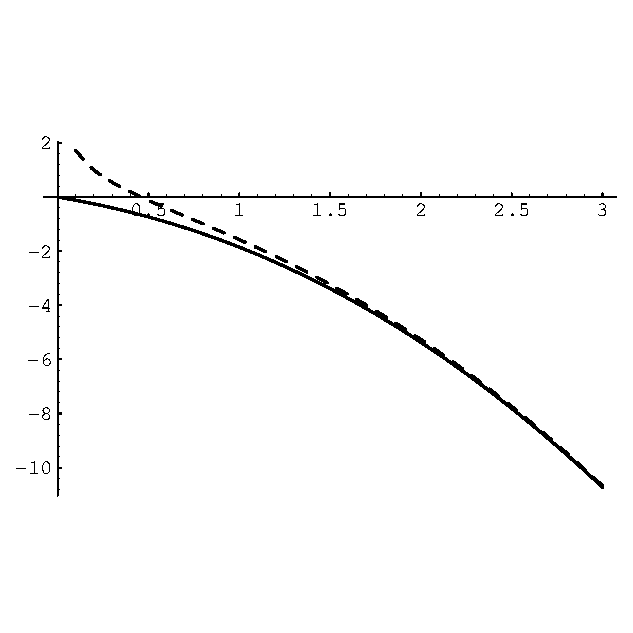
\includegraphics[width=0.6\textwidth]{ode/asymptotic/log_ft}
    \end{center}
    \caption{The logarithm of the approximation to the complementary error 
      function.}
    \label{log_first_term}
  \end{figure}




  If we continue integrating by parts, we might get a better approximation 
  to the complementary error function.
  \begin{align*}
    \erfc(x)
    &= \frac{1}{\sqrt{\pi}}x^{-1} \e^{-x^2} - 
    \frac{1}{\sqrt{\pi}}\int_x^\infty
    t^{-2} \e^{-t^2}\,dt \\
    &= \frac{1}{\sqrt{\pi}}x^{-1} \e^{-x^2} - 
    \frac{1}{\sqrt{\pi}}\left[-\frac{1}{2}t^{-3}\e^{-t^2}
    \right]_x^\infty
    + \frac{1}{\sqrt{\pi}}\int_x^\infty
    \frac{3}{2}t^{-4} \e^{-t^2}\,dt \\
    &= \frac{1}{\sqrt{\pi}}\e^{-x^2}\left(x^{-1} 
      - \frac{1}{2}x^{-3}\right)
    + \frac{1}{\sqrt{\pi}}\int_x^\infty
    \frac{3}{2}t^{-4} \e^{-t^2}\,dt \\
    &= \frac{1}{\sqrt{\pi}}\e^{-x^2}\left(x^{-1} 
      - \frac{1}{2}x^{-3}\right)
    + \frac{1}{\sqrt{\pi}}\left[-\frac{3}{4}t^{-5}\e^{-t^2}
    \right]_x^\infty
    - \frac{1}{\sqrt{\pi}}\int_x^\infty
    \frac{15}{4}t^{-6} \e^{-t^2}\,dt \\
    &= \frac{1}{\sqrt{\pi}}\e^{-x^2}\left(x^{-1} 
      - \frac{1}{2}x^{-3} + \frac{3}{4}x^{-5}\right)
    - \frac{1}{\sqrt{\pi}}\int_x^\infty
    \frac{15}{4}t^{-6} \e^{-t^2}\,dt 
  \end{align*}
  The error in approximating $\erfc(x)$ with the first three terms is
  given in Table~\ref{table_ltt}.
  We see that for $x \geq 2$ the three terms give a much better approximation
  to $\erfc(x)$ than just the first term.

  \begin{table}
    \[
    \begin{array}{llll}
      \mathbf{x}      &\mathbf{\berfc(x)}     
      & \mathrm{One Term Relative Error} \qquad
      & \mathrm{Three Term Relative Error} \\
      \hline
      1       &0.157                  &0.3203         &0.6497 \\
      2       &0.00468                &0.1044         &0.0182 \\
      3       &2.21\times 10^{-5}  &0.0507         &0.0020 \\
      4       &1.54\times 10^{-8}  &0.0296         &3.9 \cdot 10^{-4} \\
      5       &1.54\times 10^{-12} &0.0192         &1.1 \cdot 10^{-4}\\
      6       &2.15\times 10^{-17} &0.0135         &3.7 \cdot 10^{-5}\\
      7       &4.18\times 10^{-23} &0.0100         &1.5 \cdot 10^{-5}\\
      8       &1.12\times 10^{-29} &0.0077         &6.9 \cdot 10^{-6}\\
      9       &4.14\times 10^{-37} &0.0061         &3.4 \cdot 10^{-6}\\
      10 \quad &2.09\times 10^{-45}\quad &0.0049 
      &1.8 \cdot 10^{-6}
    \end{array}
    \]
    \caption{The error in approximating the complementary error function.}
    \label{table_ltt}
  \end{table}


  At this point you might guess that you could continue this process 
  indefinitely.  By repeated application of integration by parts, you can
  obtain the series expansion
  \[ \erfc(x) = \frac{2}{\sqrt{\pi}} \e^{-x^2} \sum_{n=0}^\infty 
  \frac{(-1)^n (2n)!}{n! (2x)^{2n+1}}.\]
  This is a Taylor expansion about infinity.  Let's find the radius of 
  convergence.
  \begin{align*}
    \lim_{n \to \infty} \left| \frac{a_{n+1}(x)}{a_n(x)}\right| < 1 
    &\to \lim_{n \to \infty} \left| \frac{(-1)^{n+1} (2(n+1))!}
      {(n+1)! (2x)^{2(n+1)+1}} \frac{n! (2x)^{2n+1}}{(-1)^n (2n)!}
    \right| < 1 \\
    &\to \lim_{n \to \infty} \left|\frac{(2n+2)(2n+1)}{(n+1)(2x)^2}\right|
    < 1 \\
    &\to \lim_{n \to \infty} \left|\frac{2(2n+1)}{(2x)^2}\right| < 1 \\
    &\to \left| \frac{1}{x}\right| = 0
  \end{align*}
  Thus we see that our series diverges for all $x$.  Our conventional 
  mathematical sense would tell us that this series is useless, however we
  will see that this series is very useful as an asymptotic expansion of
  $\erfc(x)$.  

  Say we are working with a convergent series expansion of some function $f(x)$.
  \[f(x) = \sum_{n=0}^\infty a_n(x)\]
  For fixed $x=x_0$, 
  \[ f(x_0) - \sum_{n=0}^N a_n(x_0) \to 0 \quad \mathrm{as}\ N \to \infty.\]
  For an asymptotic series we have a quite different behavior.
  If $g(x)$ is asymptotic to $\sum_{n = 0}^\infty b_n(x)$ as $x \to x_0$ then
  for fixed $N$,
  \[ g(x) - \sum_0^N b_n(x) \ll b_N(x) \quad \mathrm{as}\ x \to x_0. \]
  For the complementary error function,
  \[\mathrm{For fixed}\ N,\ \erfc(x) - \frac{2}{\sqrt{\pi}} \e^{-x^2} 
  \sum_{n=0}^N \frac{(-1)^n (2n)!}{n! (2x)^{2n+1}} \ll x^{-2N-1} \quad
  \mathrm{as}\ x \to \infty.\]
  We say that the error function is asymptotic to the series as $x$ goes to 
  infinity.
  \[ \erfc(x) \sim \frac{2}{\sqrt{\pi}} \e^{-x^2} \sum_{n=0}^\infty 
  \frac{(-1)^n (2n)!}{n! (2x)^{2n+1}} \quad \mathrm{as}\ x \to \infty\]

  In Figure~\ref{one_ten_twenty} the logarithm of the difference between the one
  term, ten term and twenty term approximations and the complementary
  error function are graphed in coarse, medium, and fine dashed lines,
  respectively.




  \begin{figure}[h!]
    \begin{center}
      \includegraphics[width=0.6\textwidth]{ode/asymptotic/one1020}
    \end{center}
    \caption{The logarithm of the error in the approximation.}
    \label{one_ten_twenty}
  \end{figure}


  

  \paragraph{*Optimal Asymptotic Series.}
  Of the three approximations, the one term is best for $x \lesssim 2$,
  the ten term is best for $2 \lesssim x \lesssim 4$, and the twenty term
  is best for $4 \lesssim x$.  This leads us to the concept of an optimal
  asymptotic approximation.  An optimal asymptotic approximation contains 
  the number of terms in the series that best approximates the true 
  behavior.
  \index{optimal asymptotic approximations}

  In Figure~\ref{optimal} we see a plot of the number of terms in the
  approximation versus the logarithm of the error for $x = 3$.  Thus 
  we see that the optimal asymptotic approximation is the
  first nine terms.  After nine terms the error gets larger.  It was
  inevitable that the error would start to grow after some point as the
  series diverges for all $x$.


  \begin{figure}[h!]
    \begin{center}
      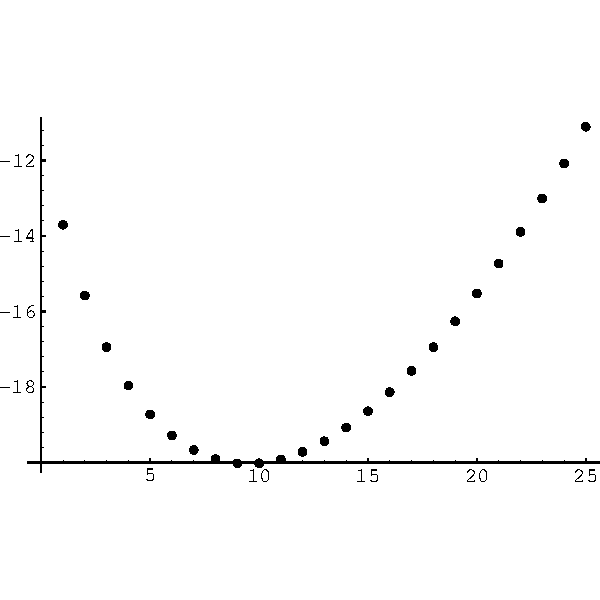
\includegraphics[width=0.6\textwidth]{ode/asymptotic/optimal}
    \end{center}
    \caption{The logarithm of the error.}
    \label{optimal}
  \end{figure}




  A good rule of thumb for finding the optimal series is to find the
  smallest term in the series and take all of the terms up to but not
  including the smallest term as the optimal approximation.  This
  makes sense, because the $n^{t h}$ term is an approximation of the
  error incurred by using the first $n-1$ terms.
  In Figure~\ref{log_nth_term} there is a plot of $n$ versus the
  logarithm of the $n^{t h}$ term in the asymptotic expansion of
  $\erfc(3)$.  We see that the tenth term is the smallest.
  Thus, in this case, our rule of thumb predicts the actual optimal series.




  \begin{figure}[h!]
    \begin{center}
      \includegraphics[width=0.6\textwidth]{ode/asymptotic/log_nt}
    \end{center}
    \caption{The logarithm of the terms in the expansion.}
    \label{log_nth_term}
  \end{figure}




\end{Example}




%%=============================================================================
\section{Asymptotic Series}

A function $f(x)$ has an asymptotic series expansion about $x=x_0$, 
$\sum_{n=0}^\infty a_n(x)$, if
\[ f(x) - \sum_{n=0}^N a_n(x) \ll a_N(x) \quad \mathrm{as}\ x \to x_0 \quad
\mathrm{for all}\ N.\]
An asymptotic series may be convergent or divergent.  Most of the 
asymptotic series you encounter will be divergent.  If the series is
convergent, then we have that
\[ f(x) - \sum_{n=0}^N a_n(x) \to 0 \quad \mathrm{as}\ N \to \infty
\quad \mathrm{for fixed}\ x.\]




Let $\epsilon_n(x)$ be some set of gauge functions.  The example that we 
are most familiar with is $\epsilon_n(x) = x^n$.  If we say that
\[ \sum_{n=0}^\infty a_n \epsilon_n(x) \sim 
\sum_{n=0}^\infty b_n \epsilon_n(x),\]
then this means that $a_n = b_n$.























%%=============================================================================
\section{Asymptotic Expansions of Differential Equations}










\subsection{The Parabolic Cylinder Equation.}

\paragraph{Controlling Factor.}
Let us examine the behavior of the bounded solution of the parabolic 
cylinder equation as $x \to + \infty$.  
\[ y'' + \left(\nu + \frac{1}{2} - \frac{1}{4} x^2\right)y = 0\]
This equation has an irregular singular point at infinity.  
With the substitution $y = \e^s$,
the equation becomes
\[s'' + (s')^2 + \nu + \frac{1}{2} - \frac{1}{4} x^2 = 0.\]
We know that 
\[ \nu + \frac{1}{2} \ll \frac{1}{4} x^2\quad \mathrm{as}\ x \to +\infty\]
so we drop this term from the equation. Let us make the assumption that
\[ s'' \ll (s')^2\quad \mathrm{as}\ x \to +\infty.\]
Thus we are left with the equation
\begin{eqnarray*}
  (s')^2 &\sim& \frac{1}{4} x^2 \\
  s' &\sim& \pm \frac{1}{2} x \\
  s &\sim& \pm \frac{1}{4} x^2 + c \\
  s &\sim& \pm \frac{1}{4} x^2\quad \mathrm{as}\ x \to +\infty
\end{eqnarray*}
Now let's check if our assumption is consistent.  Substituting into
$s'' \ll (s')^2$ yields $1/2 \ll x^2/4\quad \mathrm{as}\ x  \to +\infty$ which 
is true.  Since the equation for $y$ is second order, we would expect that 
there are two different behaviors as $x \to +\infty$.  This is 
confirmed by the fact that we found two behaviors for $s$.  $s \sim -x^2/4$
corresponds to the solution that is bounded at $+\infty$.
Thus the controlling factor of the leading behavior is $\e^{-x^2/4}$.



\paragraph{Leading Order Behavior.}
Now we attempt to get a better approximation to $s$. We make the substitution
$s = -\frac{1}{4} x^2 + t(x)$ into the equation for $s$ where 
$t \ll x^2$ as $x \to +\infty$.
\[ -\frac{1}{2} + t'' + \frac{1}{4} x^2 - x t' + (t')^2 + \nu + \frac{1}{2}
-\frac{1}{4} x^2 = 0 \]
\[ t'' - x t' + (t')^2 + \nu = 0 \]
Since $t \ll x^2$, we assume that $t' \ll x$ and $t'' \ll 1$ as 
$x \to +\infty$.  
Note that this in only an assumption since it is not always valid to
differentiate an asymptotic relation.
Thus $(t')^2 \ll x t'$ and $t'' \ll x t'$ as
$x \to +\infty$; we drop these terms from the equation.  
\begin{eqnarray*}
  t' &\sim& \frac{\nu}{x} \\
  t &\sim& \nu \log x + c \\
  t &\sim& \nu \log x\quad \mathrm{as}\ x \to +\infty
\end{eqnarray*}
Checking our assumptions for the derivatives of $t$,
\[ t' \ll x \quad \to \quad \frac{1}{x} \ll x \qquad \qquad
t'' \ll 1 \quad \to \quad \frac{1}{x^2} \ll 1,\]
we see that they were consistent.  Now we wish to refine our approximation for
$t$ with the substitution $t(x) = \nu \log x + u(x)$.
So far we have that 
\[ y \sim \exp\left[-\frac{x^2}{4} + \nu \log x + u(x)\right] 
= x^\nu \exp\left[-\frac{x^2}{4}+ u(x) \right] 
\quad  \mathrm{as}\ x \to +\infty. \]
We can try and determine $u(x)$ by substituting the expression
$t(x) = \nu \log x + u(x)$ into the equation for $t$. 
\[ -\frac{\nu}{x^2} + u'' - (\nu + x u') + \frac{\nu^2}{x^2} + 
\frac{2\nu}{x} u' + (u')^2 + \nu = 0\]
After suitable simplification, this equation becomes
\[ u' \sim \frac{\nu^2 - \nu}{x^3}\quad \mathrm{as}\ x \to +\infty \]
Integrating this asymptotic relation, 
\[ u \sim \frac{\nu-\nu^2}{2x^2} + c \quad \mathrm{as}\ x \to +\infty. \]
Notice that $\frac{\nu-\nu^2}{2x^2} \ll c$ as $x \to +\infty$;
thus this procedure fails to give us the behavior of $u(x)$.  Further 
refinements to our approximation for $s$ go to a constant value as 
$x \to +\infty$.  Thus we have that the leading behavior is
\[y \sim c x^\nu \exp\left[-\frac{x^2}{4} \right]
\quad \mathrm{as}\ x \to +\infty\]




\paragraph{Asymptotic Expansion}
Since we have factored off the singular behavior of $y$, we might expect that
what is left over is well behaved enough to be expanded in a Taylor series
about infinity. 
Let us assume that we can expand the solution for $y$ in the form
\[ y(x) \sim x^\nu \exp\left(-\frac{x^2}{4} \right) \sigma(x) = 
x^\nu \exp\left(-\frac{x^2}{4}\right) \sum_{n=0}^\infty a_n x^{-n}
\mathrm{as}\ x \to +\infty\]
where $a_0 = 1$.
Differentiating $y = x^\nu \exp\left(-\frac{x^2}{4} \right)\sigma(x)$,
\[ y' = \left[\nu x^{\nu-1} - \frac{1}{2} x^{\nu+1}\right]\e^{-x^2/4} \sigma(x) 
+ x^\nu \e^{-x^2/4} \sigma'(x) \]
\begin{align*} 
  y'' &= \left[\nu(\nu-1)x^{\nu-2} - \frac{1}{2}\nu x^\nu 
    - \frac{1}{2}(\nu+1)x^\nu
    +\frac{1}{4}x^{\nu+2}\right]\e^{-x^2/4}\sigma(x) + 
  2\left[\nu x^{\nu-1} - \frac{1}{2} x^{\nu+1}\right]
  \e^{-x^2/4} \sigma'(x) \\
  &\qquad + x^\nu \e^{-x^2/4} \sigma''(x).
\end{align*}
Substituting this into the differential equation for $y$,
\begin{gather*}
  \left[\nu(\nu-1)x^{-2} - (\nu+\frac{1}{2}) + \frac{1}{4} x^2\right]\sigma(x) + 
  2\left[\nu x^{-1} - \frac{1}{2} x\right]\sigma'(x) + \sigma''(x) + 
  \left[\nu + \frac{1}{2} - \frac{1}{4} x^2\right]\sigma(x) = 0 \\
  \sigma''(x) + (2\nu x^{-1} - x)\sigma'(x) + \nu(\nu-1) x^{-2} \sigma = 0 \\
  x^2 \sigma''(x) + (2\nu x - x^3)\sigma'(x) + \nu(\nu-1)\sigma(x) = 0.
\end{gather*}







Differentiating the expression for $\sigma(x)$,
\begin{align*}
  \sigma(x) &= \sum_{n=0}^\infty a_n x^{-n} \\
  \sigma'(x) &= \sum_{n=1}^\infty -n a_n x^{-n-1} 
  = \sum_{n=-1}^\infty -(n+2)a_{n+2} x^{-n-3} \\
  \sigma''(x) &= \sum_{n=1}^\infty n(n+1) a_n x^{-n-2}.
\end{align*}
Substituting this into the differential equation for $\sigma(x)$,
\[      \sum_{n=1}^\infty n(n+1) a_n x^{-n} + 
2\nu \sum_{n=1}^\infty -n a_n x^{-n} - 
\sum_{n=-1}^\infty -(n+2)a_{n+2} x^{-n} + 
\nu(\nu-1) \sum_{n=0}^\infty a_n x^{-n} = 0.
\]
Equating the coefficient of $x^1$ to zero yields
\[ a_1 x = 0\quad \to \quad a_1 = 0. \]
Equating the coefficient of $x^0$,
\[2 a_2 + \nu(\nu-1)a_0 = 0 \quad \to \quad 
a_2 = -\frac{1}{2}\nu(\nu-1).\]
From the coefficient of $x^{-n}$ for $n > 0$,
\begin{align*}
  n(n+1)a_n &- 2\nu n a_n + (n+2)a_{n+2} + \nu(\nu-1)a_n = 0 \\
  (n+2)a_{n+2} &= - [n(n+1) - 2\nu n + \nu(\nu-1)]a_n \\
  (n+2)a_{n+2} &= - [n^2 + n - 2\nu n + \nu(\nu-1)]a_n \\
  (n+2)a_{n+2} &= - (n-\nu)(n-\nu+1)a_n. 
\end{align*}







Thus the recursion formula for the $a_n$'s is
\[a_{n+2} = -\frac{(n-\nu)(n-\nu+1)}{n+2}a_n,\quad a_0 = 1,\ \ \ a_1 = 0. \]
The first few terms in $\sigma(x)$ are
\[\sigma(x) \sim 1 - \frac{\nu(\nu-1)}{2^1 1!}x^{-2} + 
\frac{\nu(\nu-1)(\nu-2)(\nu-3)}{2^2 2!} x^{-4} - \cdots \quad 
\mathrm{as}\ x  \to +\infty\]
If we check the radius of convergence of this series
\begin{align*}
  \lim_{n \to \infty} \left| \frac{a_{n+2} x^{-n-2}}{a_n x^{-n}}\right|<1 \quad
  &\to \quad \lim_{n \to \infty} \left| 
    -\frac{(n-\nu)(n-\nu+1)}{n+2} x^{-2} \right| < 1 \\
  &\to \quad \frac{1}{x} = 0
\end{align*}
we see that the radius of convergence is zero.  Thus if $\nu \neq 0,1,2,\ldots$
our asymptotic expansion for $y$
\[ y \sim x^\nu \e^{-x^2/4}\left[1 - \frac{\nu(\nu-1)}{2^1 1!}x^{-2} + 
  \frac{\nu(\nu-1)(\nu-2)(\nu-3)}{2^2 2!} x^{-4} - \cdots\right] \]
diverges for all x.  However this solution is still very useful. 
If we only use a finite number of terms, we will get a very good numerical 
approximation for large $x$.


In Figure~\ref{par_cyl} the one term, two term, and three term asymptotic
approximations are shown in rough, medium, and fine dashing, respectively.
The numerical solution is plotted in a solid line.

\begin{figure}[h!]
  \begin{center}
    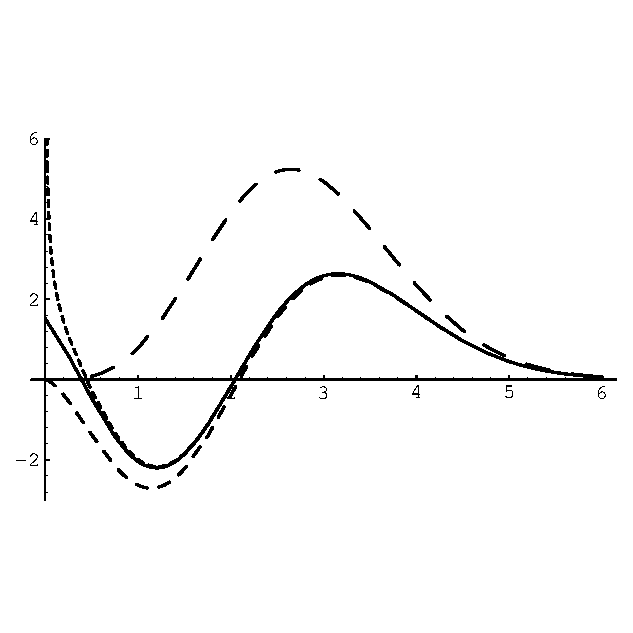
\includegraphics[width=0.6\textwidth]{ode/asymptotic/par_cyl}
  \end{center}
  \caption{Asymptotic approximations to the parabolic cylinder function.}
  \label{par_cyl}
\end{figure}










